\chapter{Results}
\label{ch:results}

%-------------------------------------------------------

This chapter shows the output of every filter, taken from the executed
notebook \texttt{notebooks/assignment2.ipynb}. Each figure shows the
original image on the left, followed by the $3 \times 3$ and the
$5 \times 5$ result.

%%%%%%%%%%%%%%%%%%%%%%%%%%%%%%%%%%%%%%%%%%%%%%%%%%%%%
\section{Input Image}
\label{sec:input}
%%%%%%%%%%%%%%%%%%%%%%%%%%%%%%%%%%%%%%%%%%%%%%%%%%%%%

\begin{figure}[H]
    \centering
    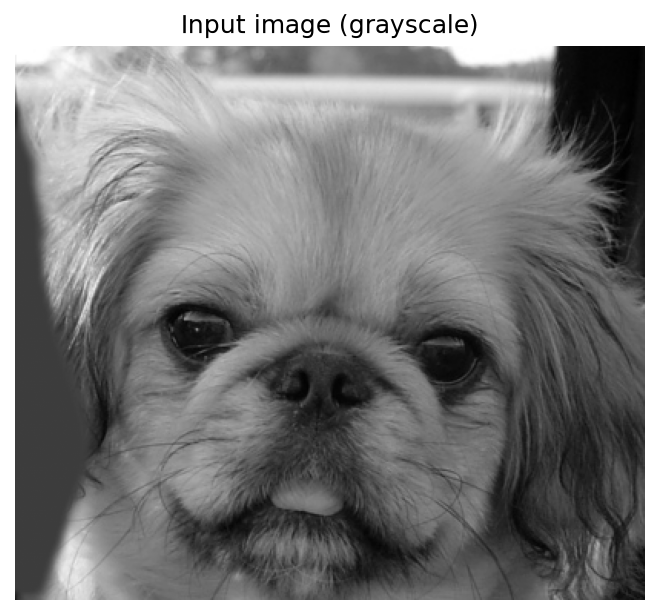
\includegraphics[width = 0.55\textwidth]{input.png}
    \caption[Input image.]%
    {Input image \texttt{dog.bmp} ($410 \times 361$), loaded in grayscale.}
    \label{fig:input}
\end{figure}


%%%%%%%%%%%%%%%%%%%%%%%%%%%%%%%%%%%%%%%%%%%%%%%%%%%%%
\section{Exercise 1 --- Box Filter without OpenCV}
\label{sec:res-ex1}
%%%%%%%%%%%%%%%%%%%%%%%%%%%%%%%%%%%%%%%%%%%%%%%%%%%%%

\begin{figure}[H]
    \centering
    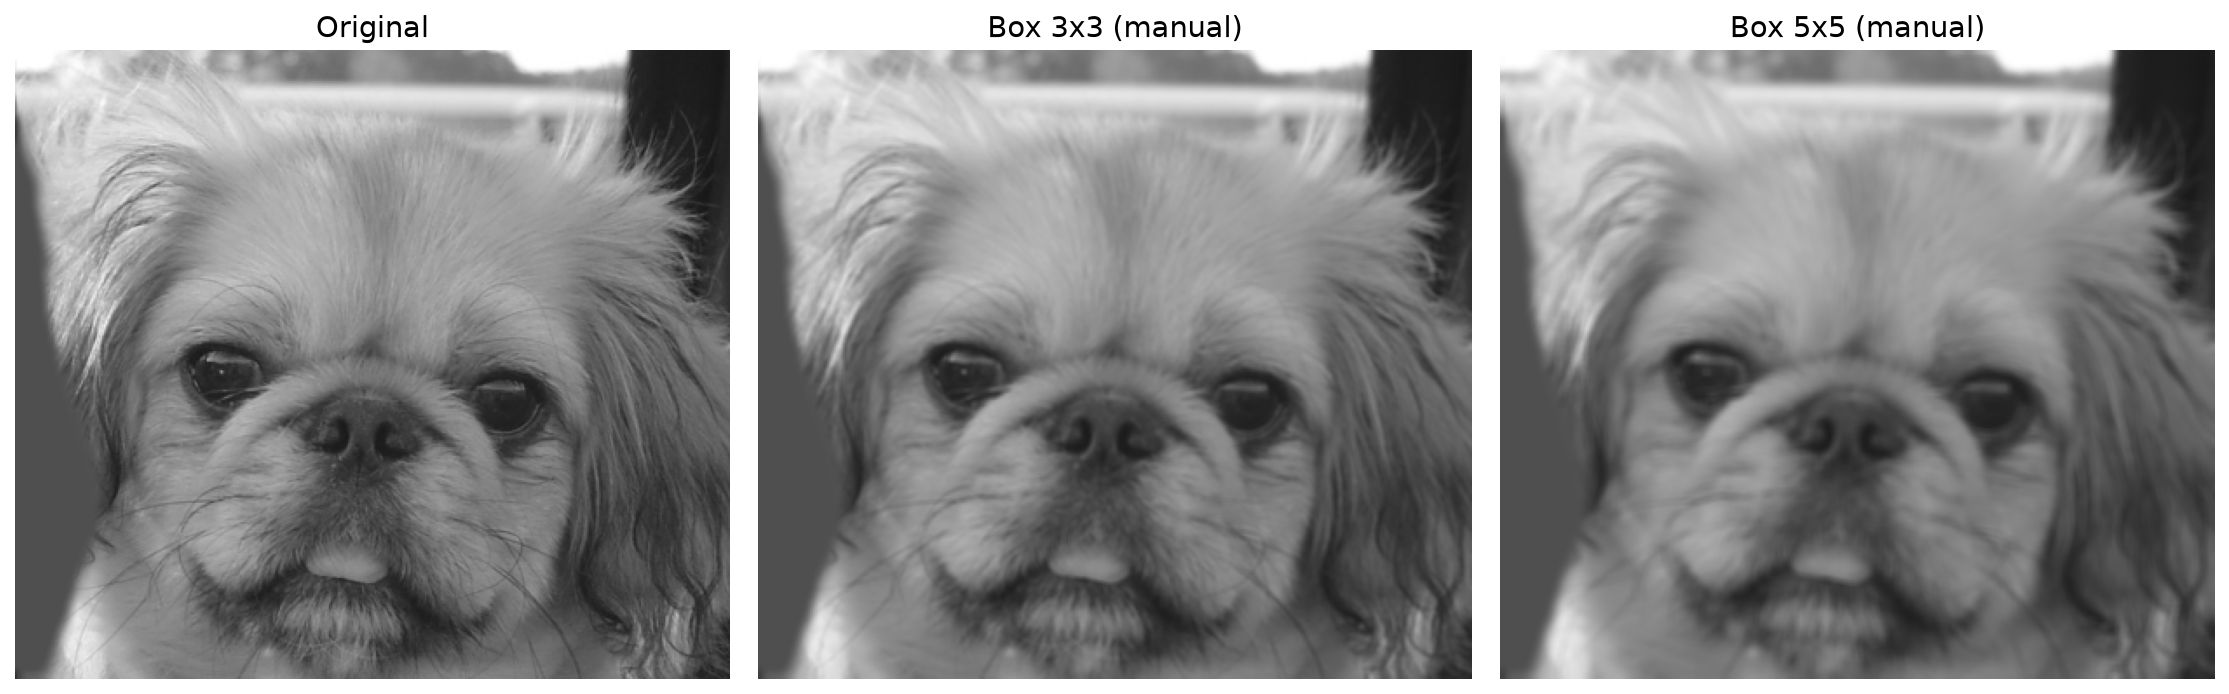
\includegraphics[width = \textwidth]{ex1_box_manual.png}
    \caption[Box filter without OpenCV.]%
    {Manual box filter with $3 \times 3$ and $5 \times 5$ kernels.}
    \label{fig:ex1}
\end{figure}

\begin{figure}[H]
    \centering
    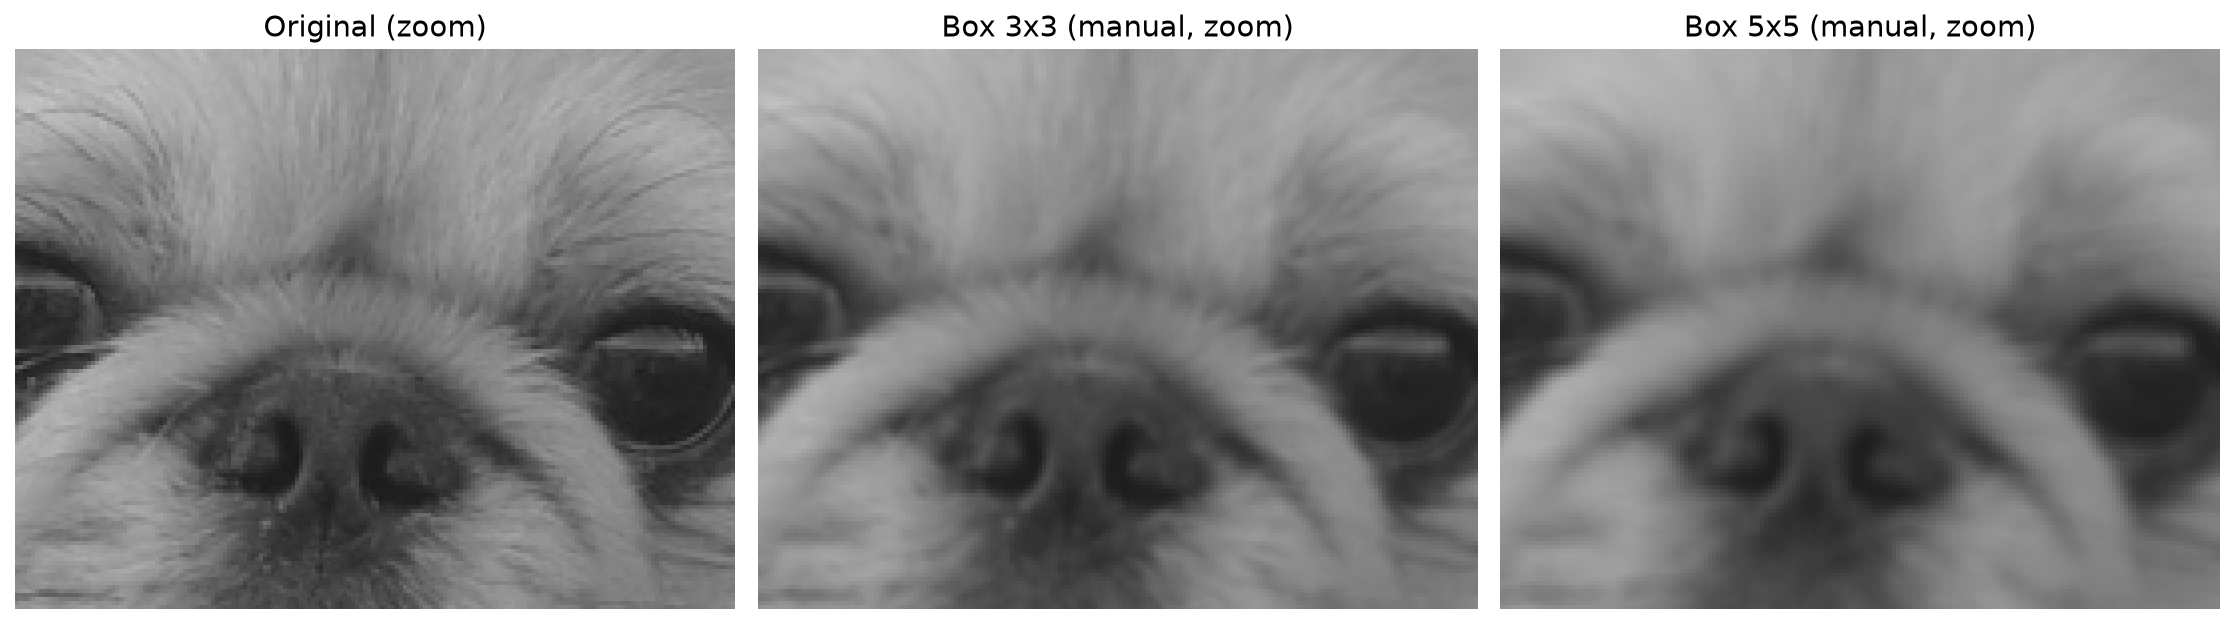
\includegraphics[width = \textwidth]{ex1_box_manual_zoom.png}
    \caption[Box filter without OpenCV (zoom).]%
    {Same results zoomed in on the eyes and nose, where the blur is
    easier to see.}
    \label{fig:ex1-zoom}
\end{figure}

\textbf{Observation.} Both kernels blur the image; the fur, whiskers and
the reflection in the eyes lose detail. The $5 \times 5$ kernel averages
25 pixels instead of 9, so it blurs noticeably more than the
$3 \times 3$ kernel. The difference is hard to see at full size but
clear in the zoomed view (Figure \ref{fig:ex1-zoom}). Each manual run
took about 0.3~s.


%%%%%%%%%%%%%%%%%%%%%%%%%%%%%%%%%%%%%%%%%%%%%%%%%%%%%
\section{Exercise 2 --- Box Filter with OpenCV}
\label{sec:res-ex2}
%%%%%%%%%%%%%%%%%%%%%%%%%%%%%%%%%%%%%%%%%%%%%%%%%%%%%

\begin{figure}[H]
    \centering
    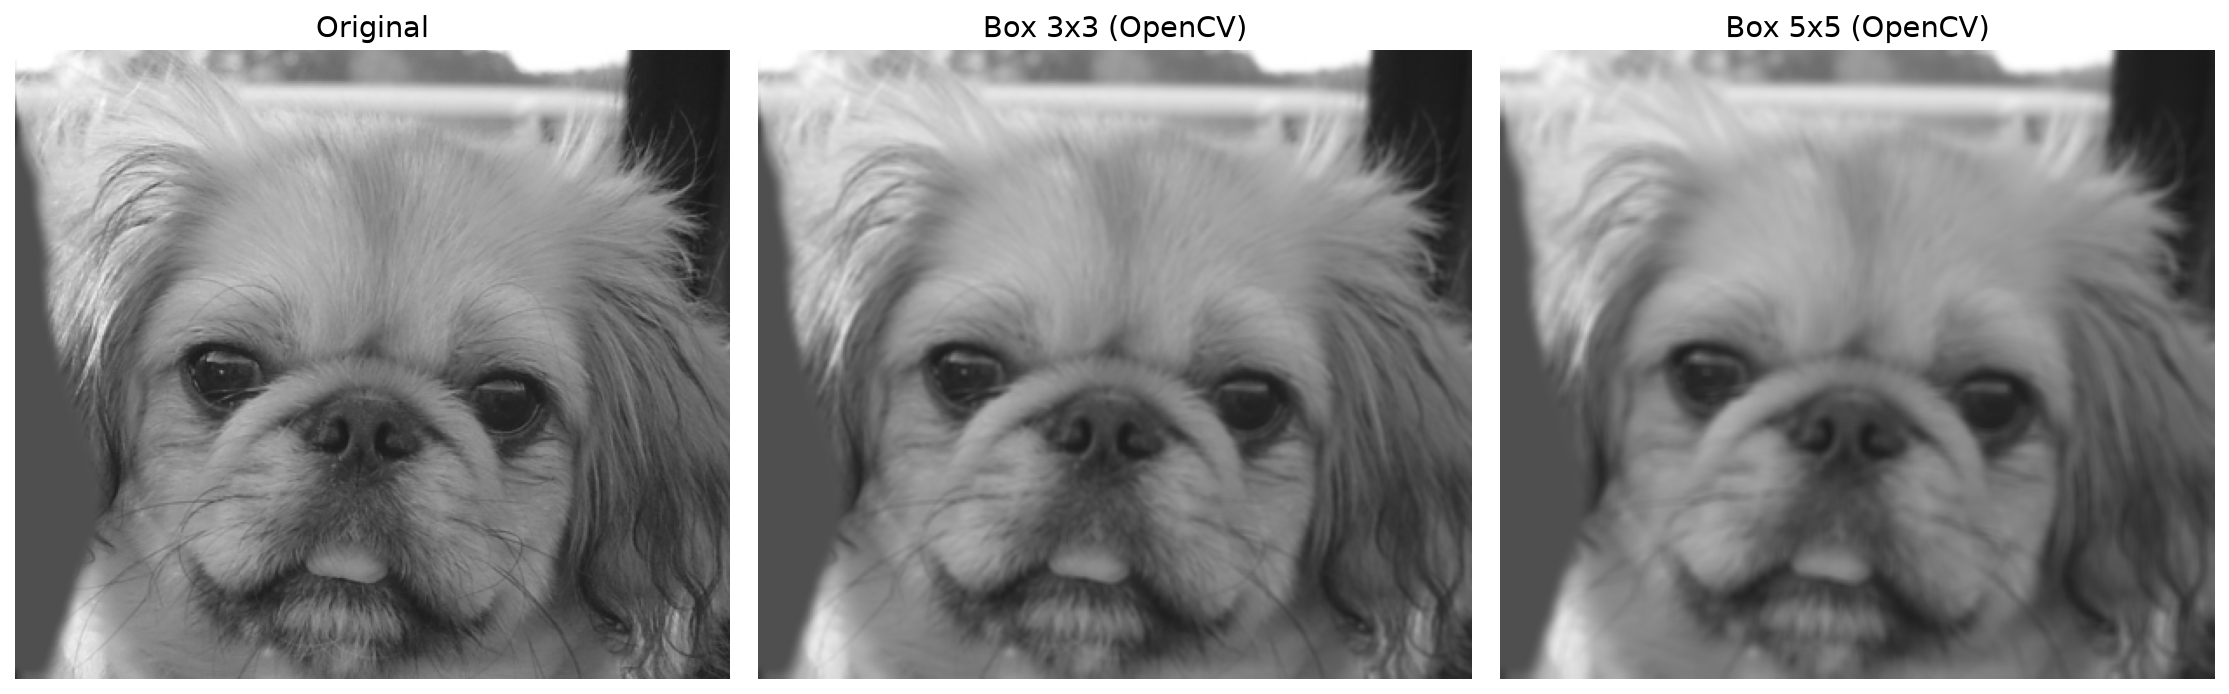
\includegraphics[width = \textwidth]{ex2_box_opencv.png}
    \caption[Box filter with OpenCV.]%
    {OpenCV box filter (\texttt{cv2.blur}) with $3 \times 3$ and
    $5 \times 5$ kernels.}
    \label{fig:ex2}
\end{figure}

\textbf{Observation.} The OpenCV output is identical to my manual
implementation: the maximum pixel difference is 0 for both kernel sizes,
including the borders, because both use reflection padding. The only
difference is speed: \texttt{cv2.blur} runs in well under a millisecond
(0.2--2~ms), while my Python loop takes about 0.3~s, which is hundreds
of times slower.


%%%%%%%%%%%%%%%%%%%%%%%%%%%%%%%%%%%%%%%%%%%%%%%%%%%%%
\section{Exercise 3 --- Sobel X without OpenCV}
\label{sec:res-ex3}
%%%%%%%%%%%%%%%%%%%%%%%%%%%%%%%%%%%%%%%%%%%%%%%%%%%%%

\begin{figure}[H]
    \centering
    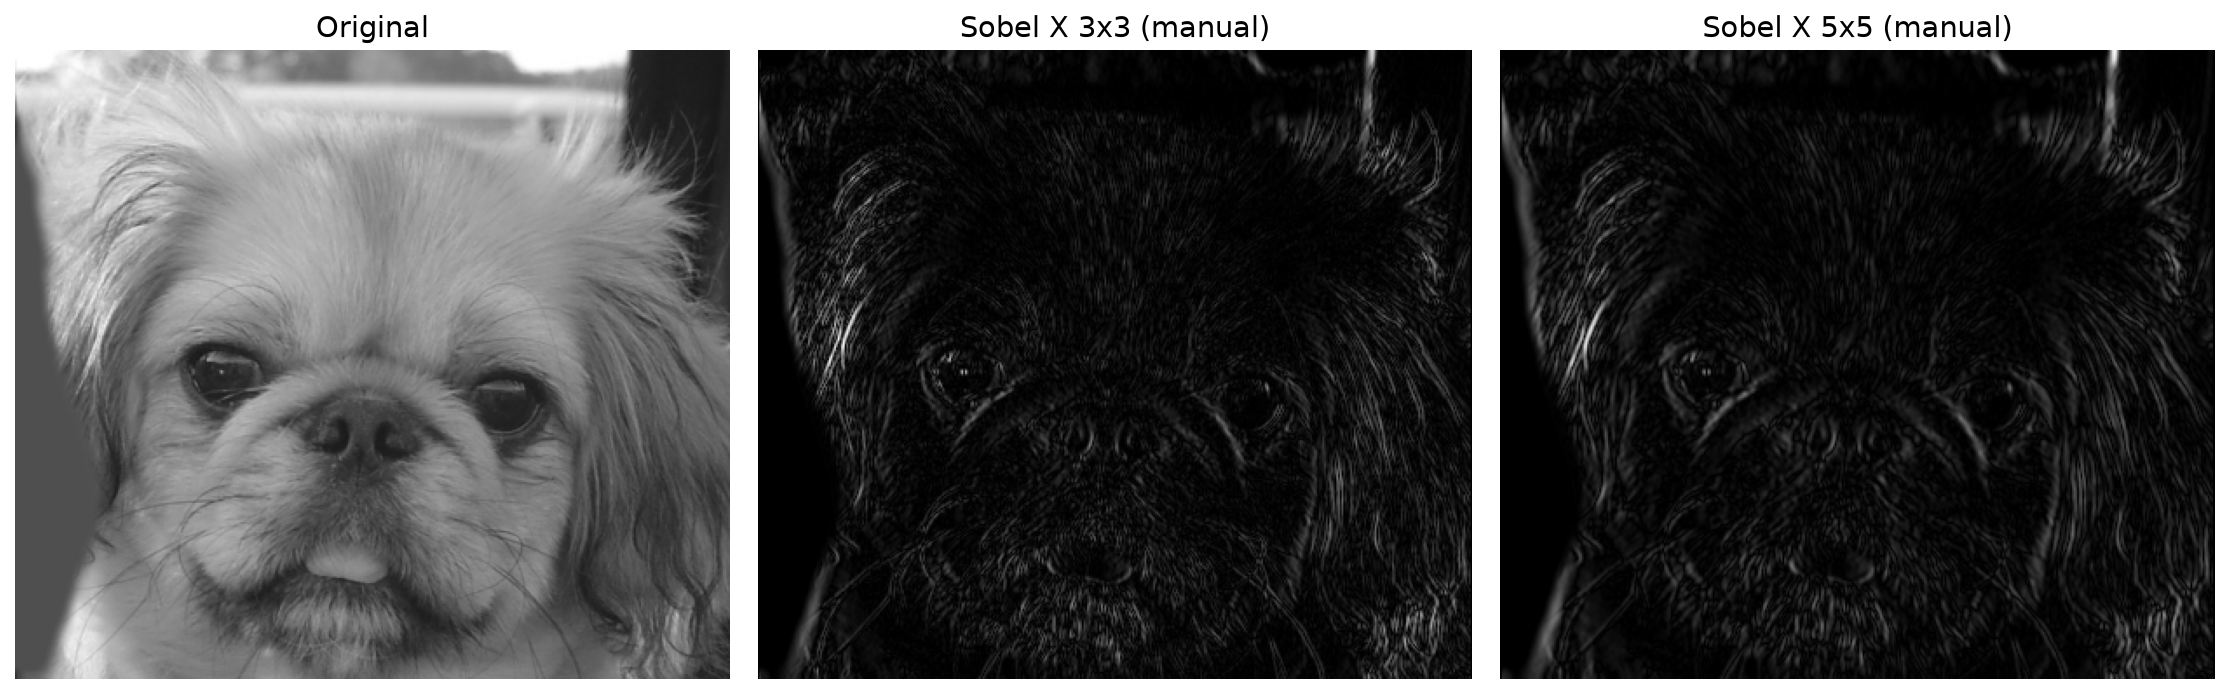
\includegraphics[width = \textwidth]{ex3_sobel_x.png}
    \caption[Sobel X without OpenCV.]%
    {Manual Sobel filter in the X direction ($|G_x|$), $3 \times 3$ and
    $5 \times 5$.}
    \label{fig:ex3}
\end{figure}

\textbf{Observation.} The X filter highlights vertical edges: the sides
of the face, the vertical strands of fur on the ears, and the vertical
post in the background at the top right. Horizontal structures, such as
the bar at the top of the image and the mouth, almost disappear. The
$3 \times 3$ result shows many thin, fine edges (and more texture
noise), while the $5 \times 5$ result gives thicker, smoother edges,
because its kernel also smooths over a wider area.


%%%%%%%%%%%%%%%%%%%%%%%%%%%%%%%%%%%%%%%%%%%%%%%%%%%%%
\section{Exercise 4 --- Sobel Y without OpenCV}
\label{sec:res-ex4}
%%%%%%%%%%%%%%%%%%%%%%%%%%%%%%%%%%%%%%%%%%%%%%%%%%%%%

\begin{figure}[H]
    \centering
    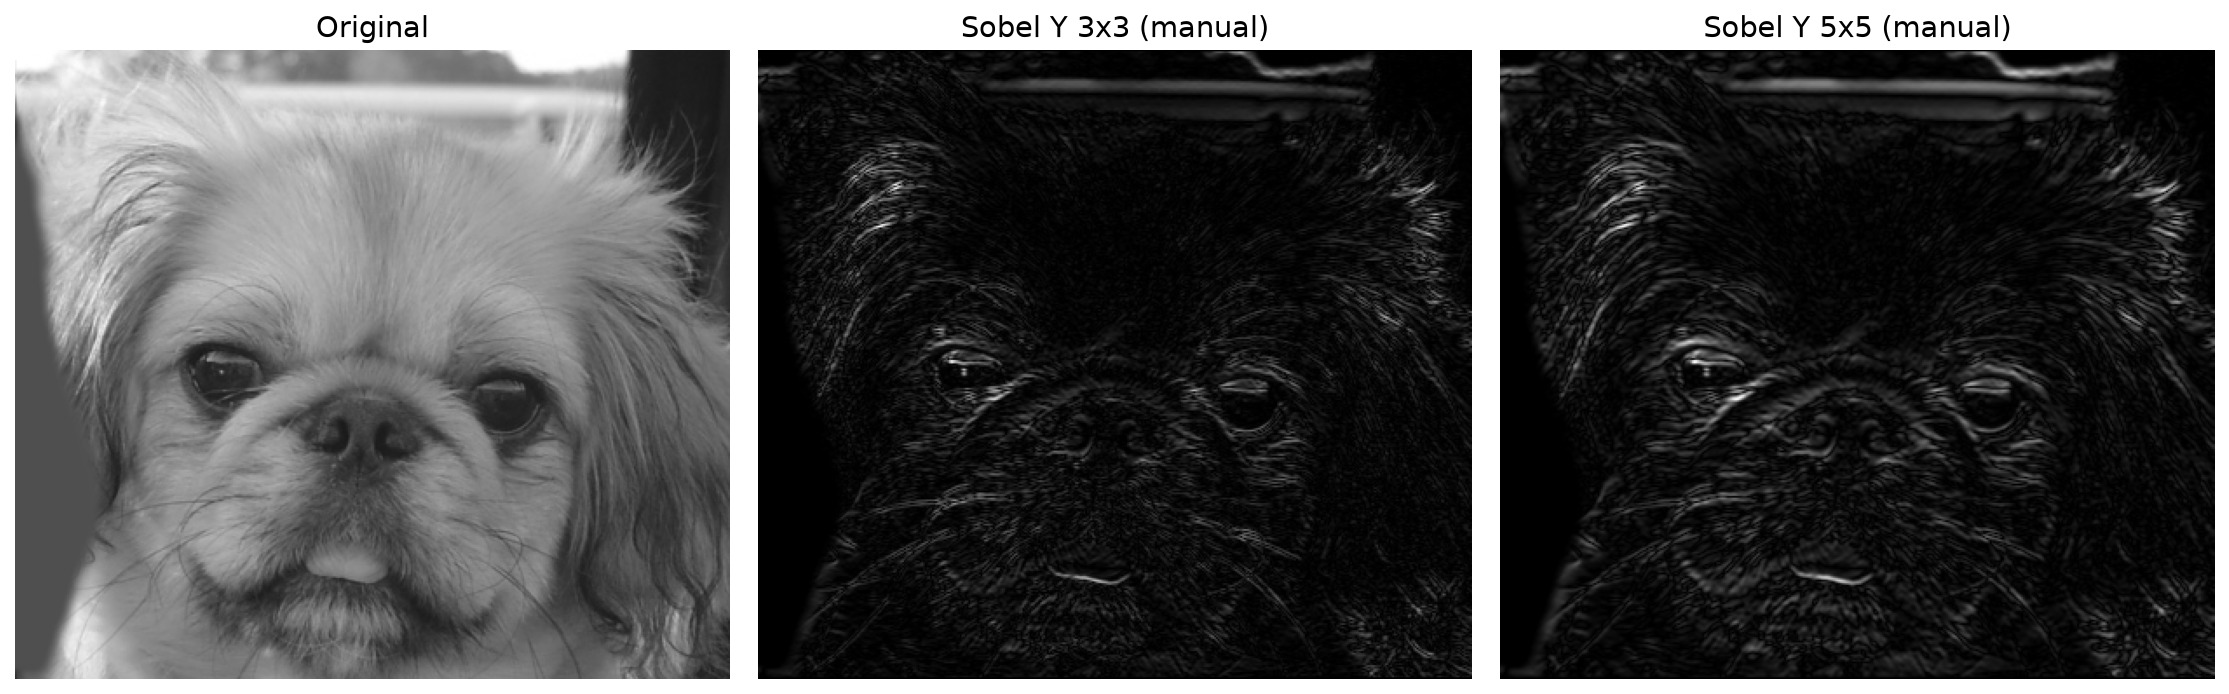
\includegraphics[width = \textwidth]{ex4_sobel_y.png}
    \caption[Sobel Y without OpenCV.]%
    {Manual Sobel filter in the Y direction ($|G_y|$), $3 \times 3$ and
    $5 \times 5$.}
    \label{fig:ex4}
\end{figure}

\textbf{Observation.} The Y filter is the opposite of the X filter: it
highlights horizontal edges, such as the bar in the background, the top
and bottom of the eyes, the nose and the mouth, while the vertical sides
of the face become weak. Again, the $5 \times 5$ kernel produces thicker
and less noisy edges than the $3 \times 3$ kernel.


%%%%%%%%%%%%%%%%%%%%%%%%%%%%%%%%%%%%%%%%%%%%%%%%%%%%%
\section{Exercise 5 --- Sobel X and Y without OpenCV}
\label{sec:res-ex5}
%%%%%%%%%%%%%%%%%%%%%%%%%%%%%%%%%%%%%%%%%%%%%%%%%%%%%

\begin{figure}[H]
    \centering
    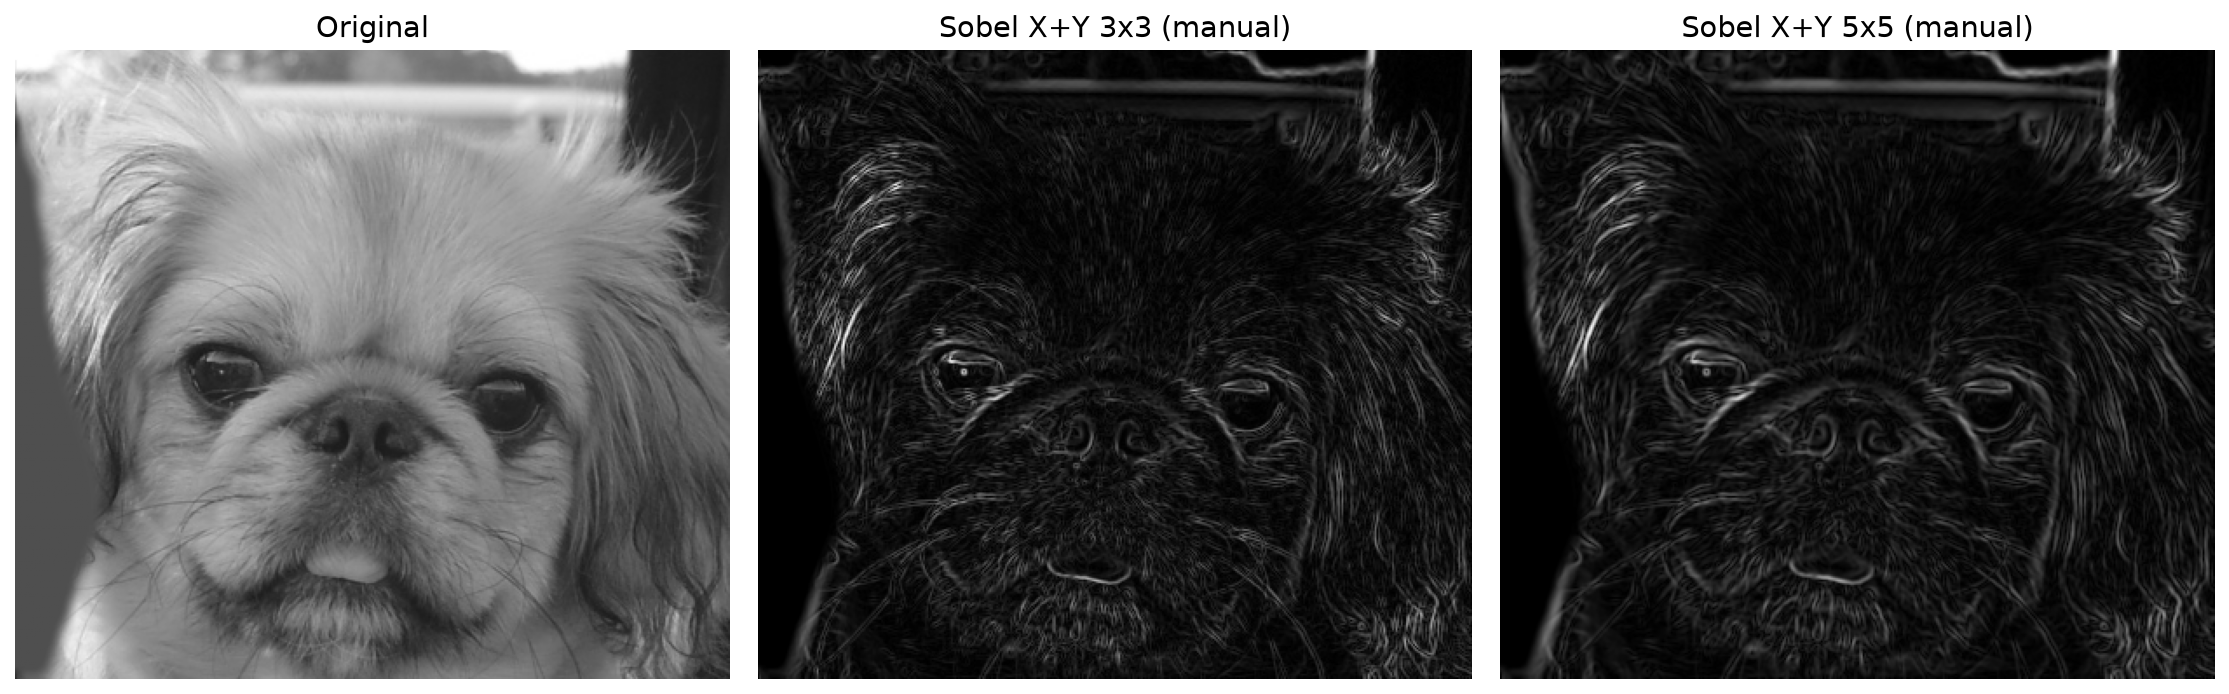
\includegraphics[width = \textwidth]{ex5_sobel_xy.png}
    \caption[Sobel X and Y without OpenCV.]%
    {Manual gradient magnitude $\sqrt{G_x^2 + G_y^2}$, $3 \times 3$ and
    $5 \times 5$.}
    \label{fig:ex5}
\end{figure}

\textbf{Observation.} Combining both directions gives a complete edge
map: the outline of the eyes, nose, mouth and fur is visible no matter
which direction the edge runs. The $3 \times 3$ magnitude is sharper and
shows more fine texture; the $5 \times 5$ magnitude is smoother and
keeps mostly the stronger edges.


%%%%%%%%%%%%%%%%%%%%%%%%%%%%%%%%%%%%%%%%%%%%%%%%%%%%%
\section{Exercise 6 --- Sobel X and Y with OpenCV}
\label{sec:res-ex6}
%%%%%%%%%%%%%%%%%%%%%%%%%%%%%%%%%%%%%%%%%%%%%%%%%%%%%

\begin{figure}[H]
    \centering
    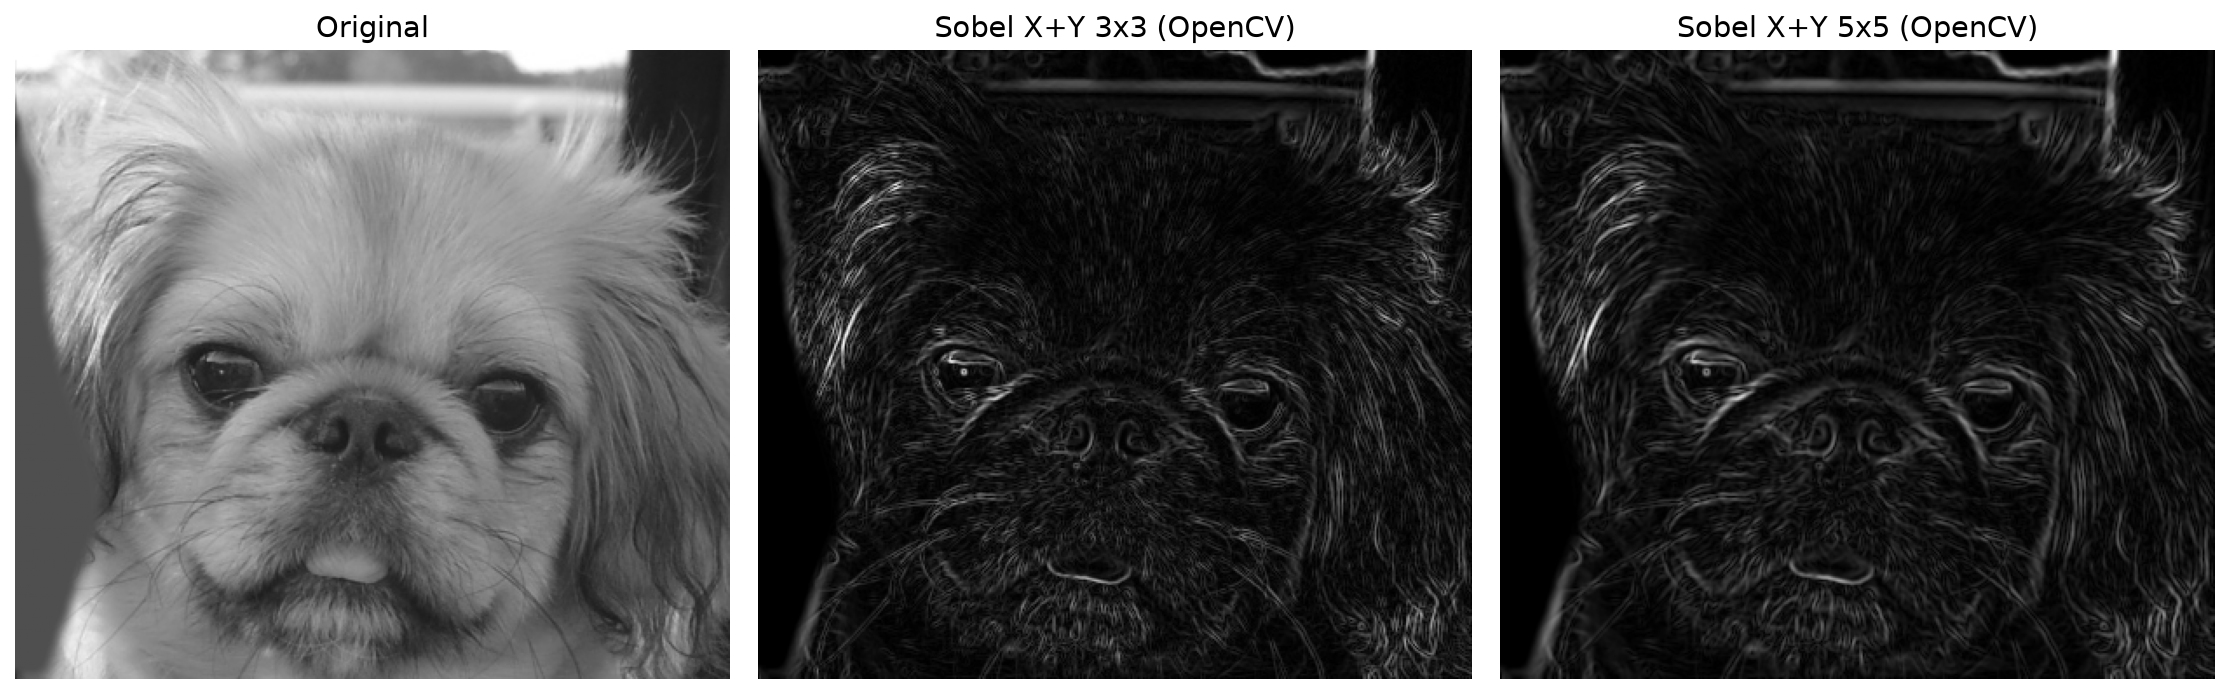
\includegraphics[width = \textwidth]{ex6_sobel_xy_opencv.png}
    \caption[Sobel X and Y with OpenCV.]%
    {Gradient magnitude computed with \texttt{cv2.Sobel} and
    \texttt{cv2.magnitude}, $3 \times 3$ and $5 \times 5$.}
    \label{fig:ex6}
\end{figure}

\textbf{Observation.} The OpenCV result matches my manual implementation
exactly (maximum difference 0.0 for both kernel sizes), which confirms
that my $3 \times 3$ and $5 \times 5$ kernels and my border handling are
the same as OpenCV's.


%%%%%%%%%%%%%%%%%%%%%%%%%%%%%%%%%%%%%%%%%%%%%%%%%%%%%
\section{Exercise 7 --- Gaussian Filter with OpenCV}
\label{sec:res-ex7}
%%%%%%%%%%%%%%%%%%%%%%%%%%%%%%%%%%%%%%%%%%%%%%%%%%%%%

\begin{figure}[H]
    \centering
    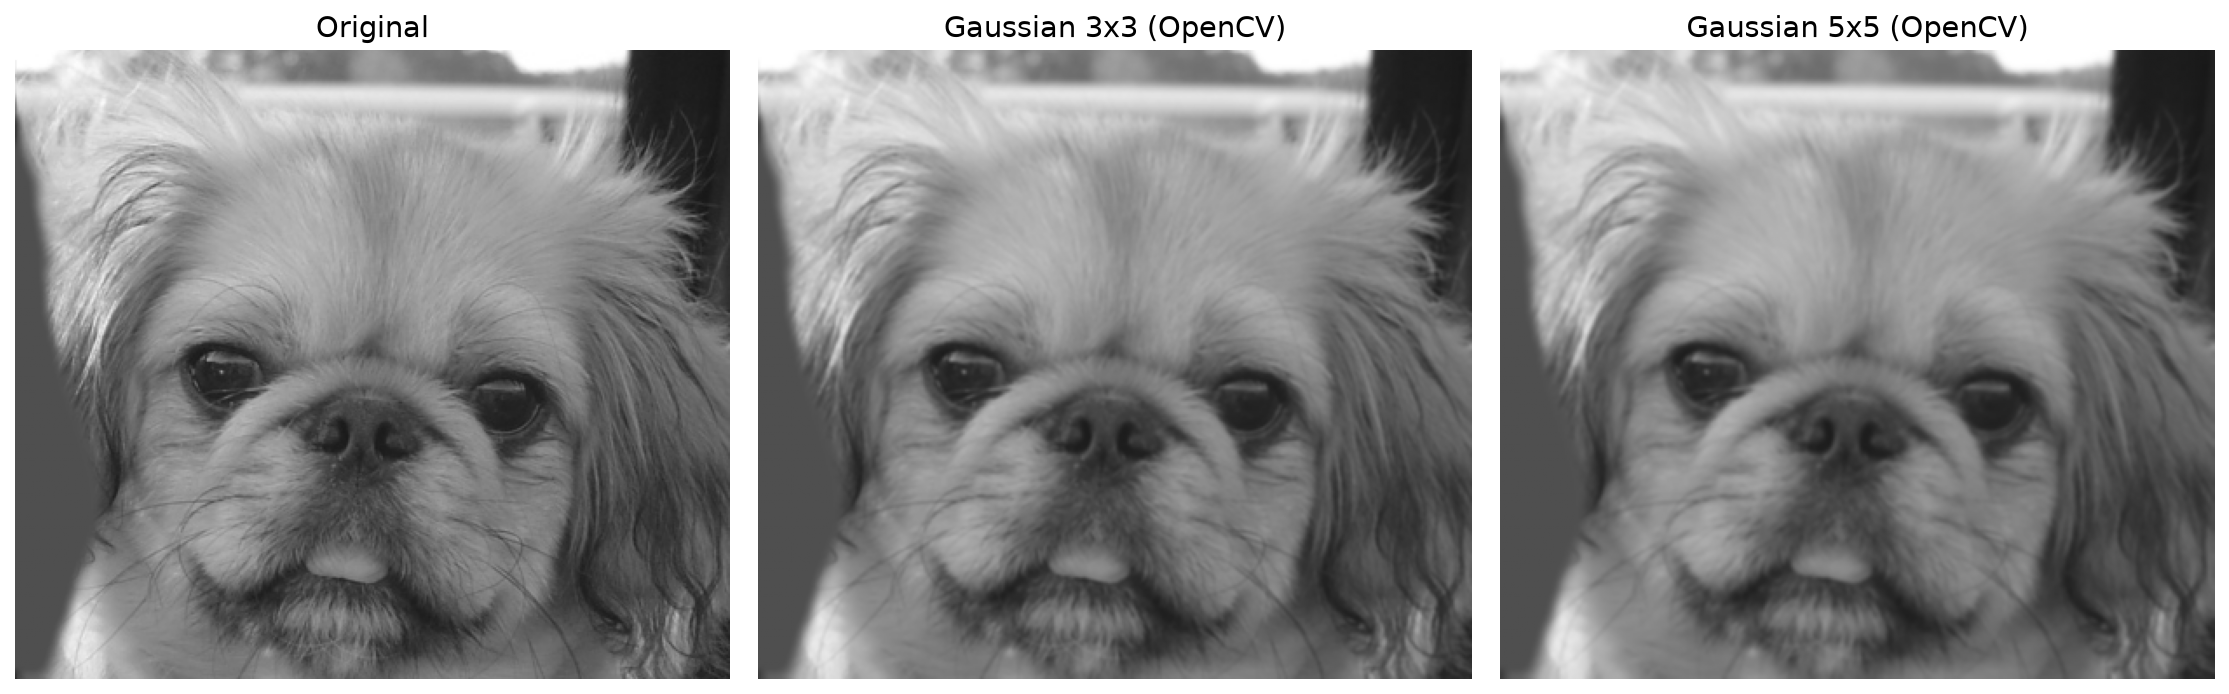
\includegraphics[width = \textwidth]{ex7_gaussian.png}
    \caption[Gaussian filter with OpenCV.]%
    {Gaussian filter (\texttt{cv2.GaussianBlur}, $\sigma = 0$),
    $3 \times 3$ and $5 \times 5$.}
    \label{fig:ex7}
\end{figure}

\begin{figure}[H]
    \centering
    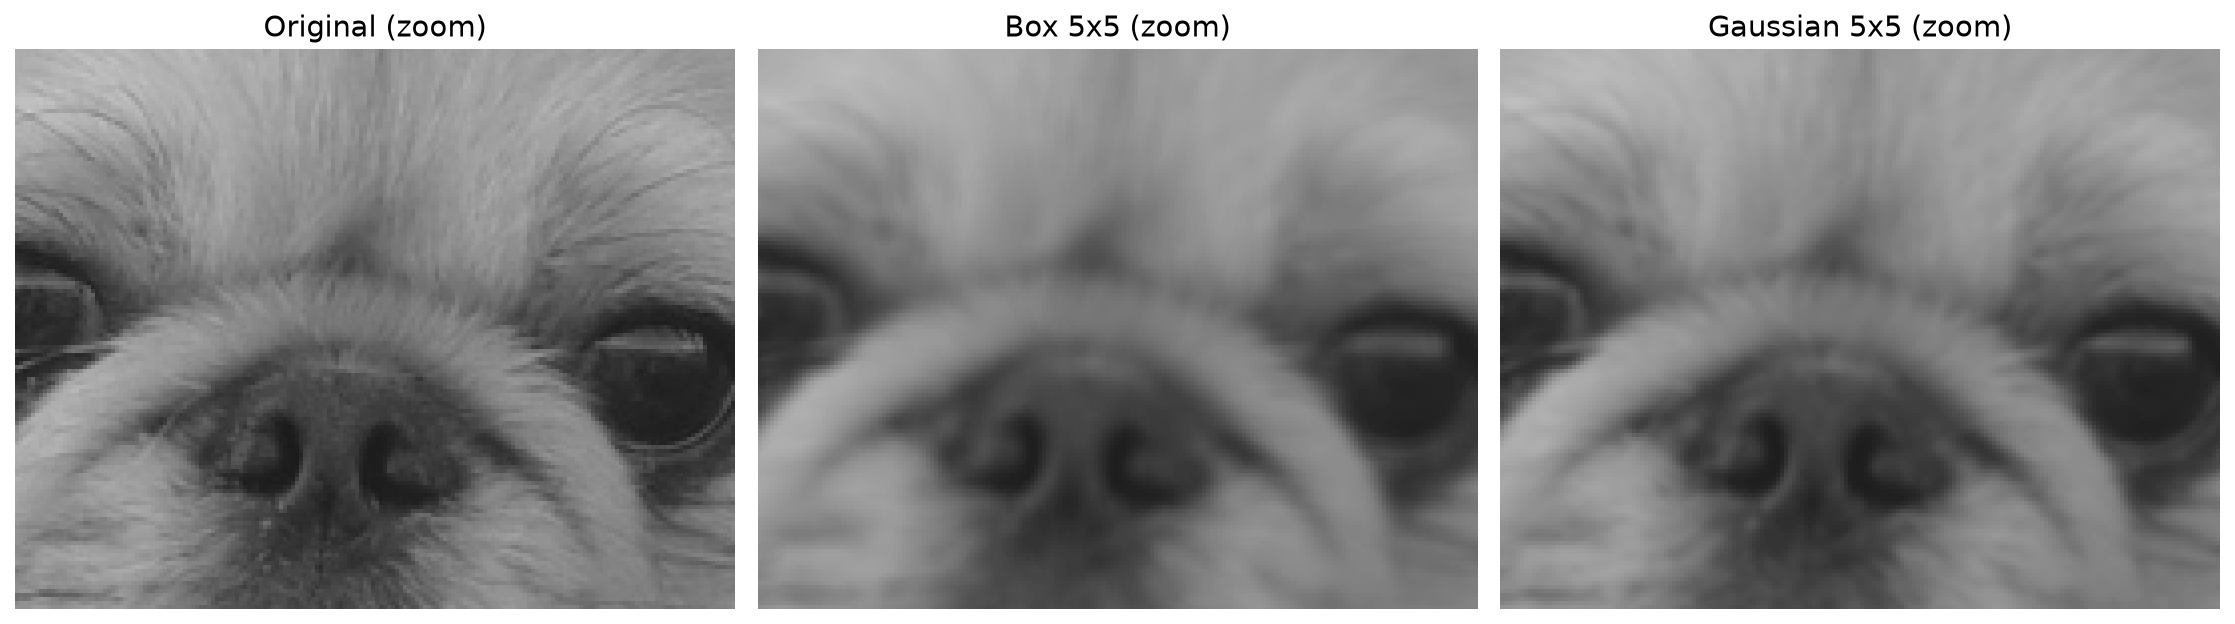
\includegraphics[width = \textwidth]{ex7_box_vs_gaussian_zoom.png}
    \caption[Box filter vs.\ Gaussian filter (zoom).]%
    {Box filter and Gaussian filter with the same $5 \times 5$ kernel
    size, zoomed in on the eyes and nose.}
    \label{fig:ex7-zoom}
\end{figure}

\textbf{Observation.} The Gaussian filter also smooths the image, but
with the same kernel size it blurs less than the box filter and keeps
the edges more natural (Figure \ref{fig:ex7-zoom}). This is because the
center pixel has the largest weight and the pixels further away count
less, while the box filter gives the same weight to every pixel in the
window. As with the box filter, the $5 \times 5$ kernel blurs more than
the $3 \times 3$ kernel.
